\documentclass[11pt,a4paper]{report}
\usepackage[textwidth=37em,vmargin=30mm]{geometry}
\usepackage{calc,xunicode,amsmath,amssymb,paralist,enumitem,tabu,booktabs,datetime2,xeCJK,xeCJKfntef,listings}
\usepackage{tocloft,fancyhdr,tcolorbox,xcolor,graphicx,eso-pic,xltxtra,xelatexemoji}

\newcommand{\envyear}[0]{2024}
\newcommand{\envdatestr}[0]{2024-12-29}
\newcommand{\envfinaldir}[0]{webdb/2024/20241229/final}

\usepackage[hidelinks]{hyperref}
\hypersetup{
    colorlinks=false,
    pdfpagemode=FullScreen,
    pdftitle={Web Digest - \envdatestr}
}

\setlength{\cftbeforechapskip}{10pt}
\renewcommand{\cftchapfont}{\rmfamily\bfseries\large\raggedright}
\setlength{\cftbeforesecskip}{2pt}
\renewcommand{\cftsecfont}{\sffamily\small\raggedright}

\setdefaultleftmargin{2em}{2em}{1em}{1em}{1em}{1em}

\usepackage{xeCJK,xeCJKfntef}
\xeCJKsetup{PunctStyle=plain,RubberPunctSkip=false,CJKglue=\strut\hskip 0pt plus 0.1em minus 0.05em,CJKecglue=\strut\hskip 0.22em plus 0.2em}
\XeTeXlinebreaklocale "zh"
\XeTeXlinebreakskip = 0pt


\setmainfont{Brygada 1918}
\setromanfont{Brygada 1918}
\setsansfont{IBM Plex Sans}
\setmonofont{JetBrains Mono NL}
\setCJKmainfont{Noto Serif CJK SC}
\setCJKromanfont{Noto Serif CJK SC}
\setCJKsansfont{Noto Sans CJK SC}
\setCJKmonofont{Noto Sans CJK SC}

\setlength{\parindent}{0pt}
\setlength{\parskip}{8pt}
\linespread{1.15}

\lstset{
	basicstyle=\ttfamily\footnotesize,
	numbersep=5pt,
	backgroundcolor=\color{black!5},
	showspaces=false,
	showstringspaces=false,
	showtabs=false,
	tabsize=2,
	captionpos=b,
	breaklines=true,
	breakatwhitespace=true,
	breakautoindent=true,
	linewidth=\textwidth
}






\newcommand{\coverpic}[2]{
    % argv: itemurl, authorname
    Cover photo by #2~~(\href{#1}{#1})
}
\newcommand{\makeheader}[0]{
    \begin{titlepage}
        % \newgeometry{hmargin=15mm,tmargin=21mm,bmargin=12mm}
        \begin{center}
            
            \rmfamily\scshape
            \fontspec{BaskervilleF}
            \fontspec{Old Standard}
            \fontsize{59pt}{70pt}\selectfont
            WEB\hfill DIGEST
            
            \vfill
            % \vskip 30pt
            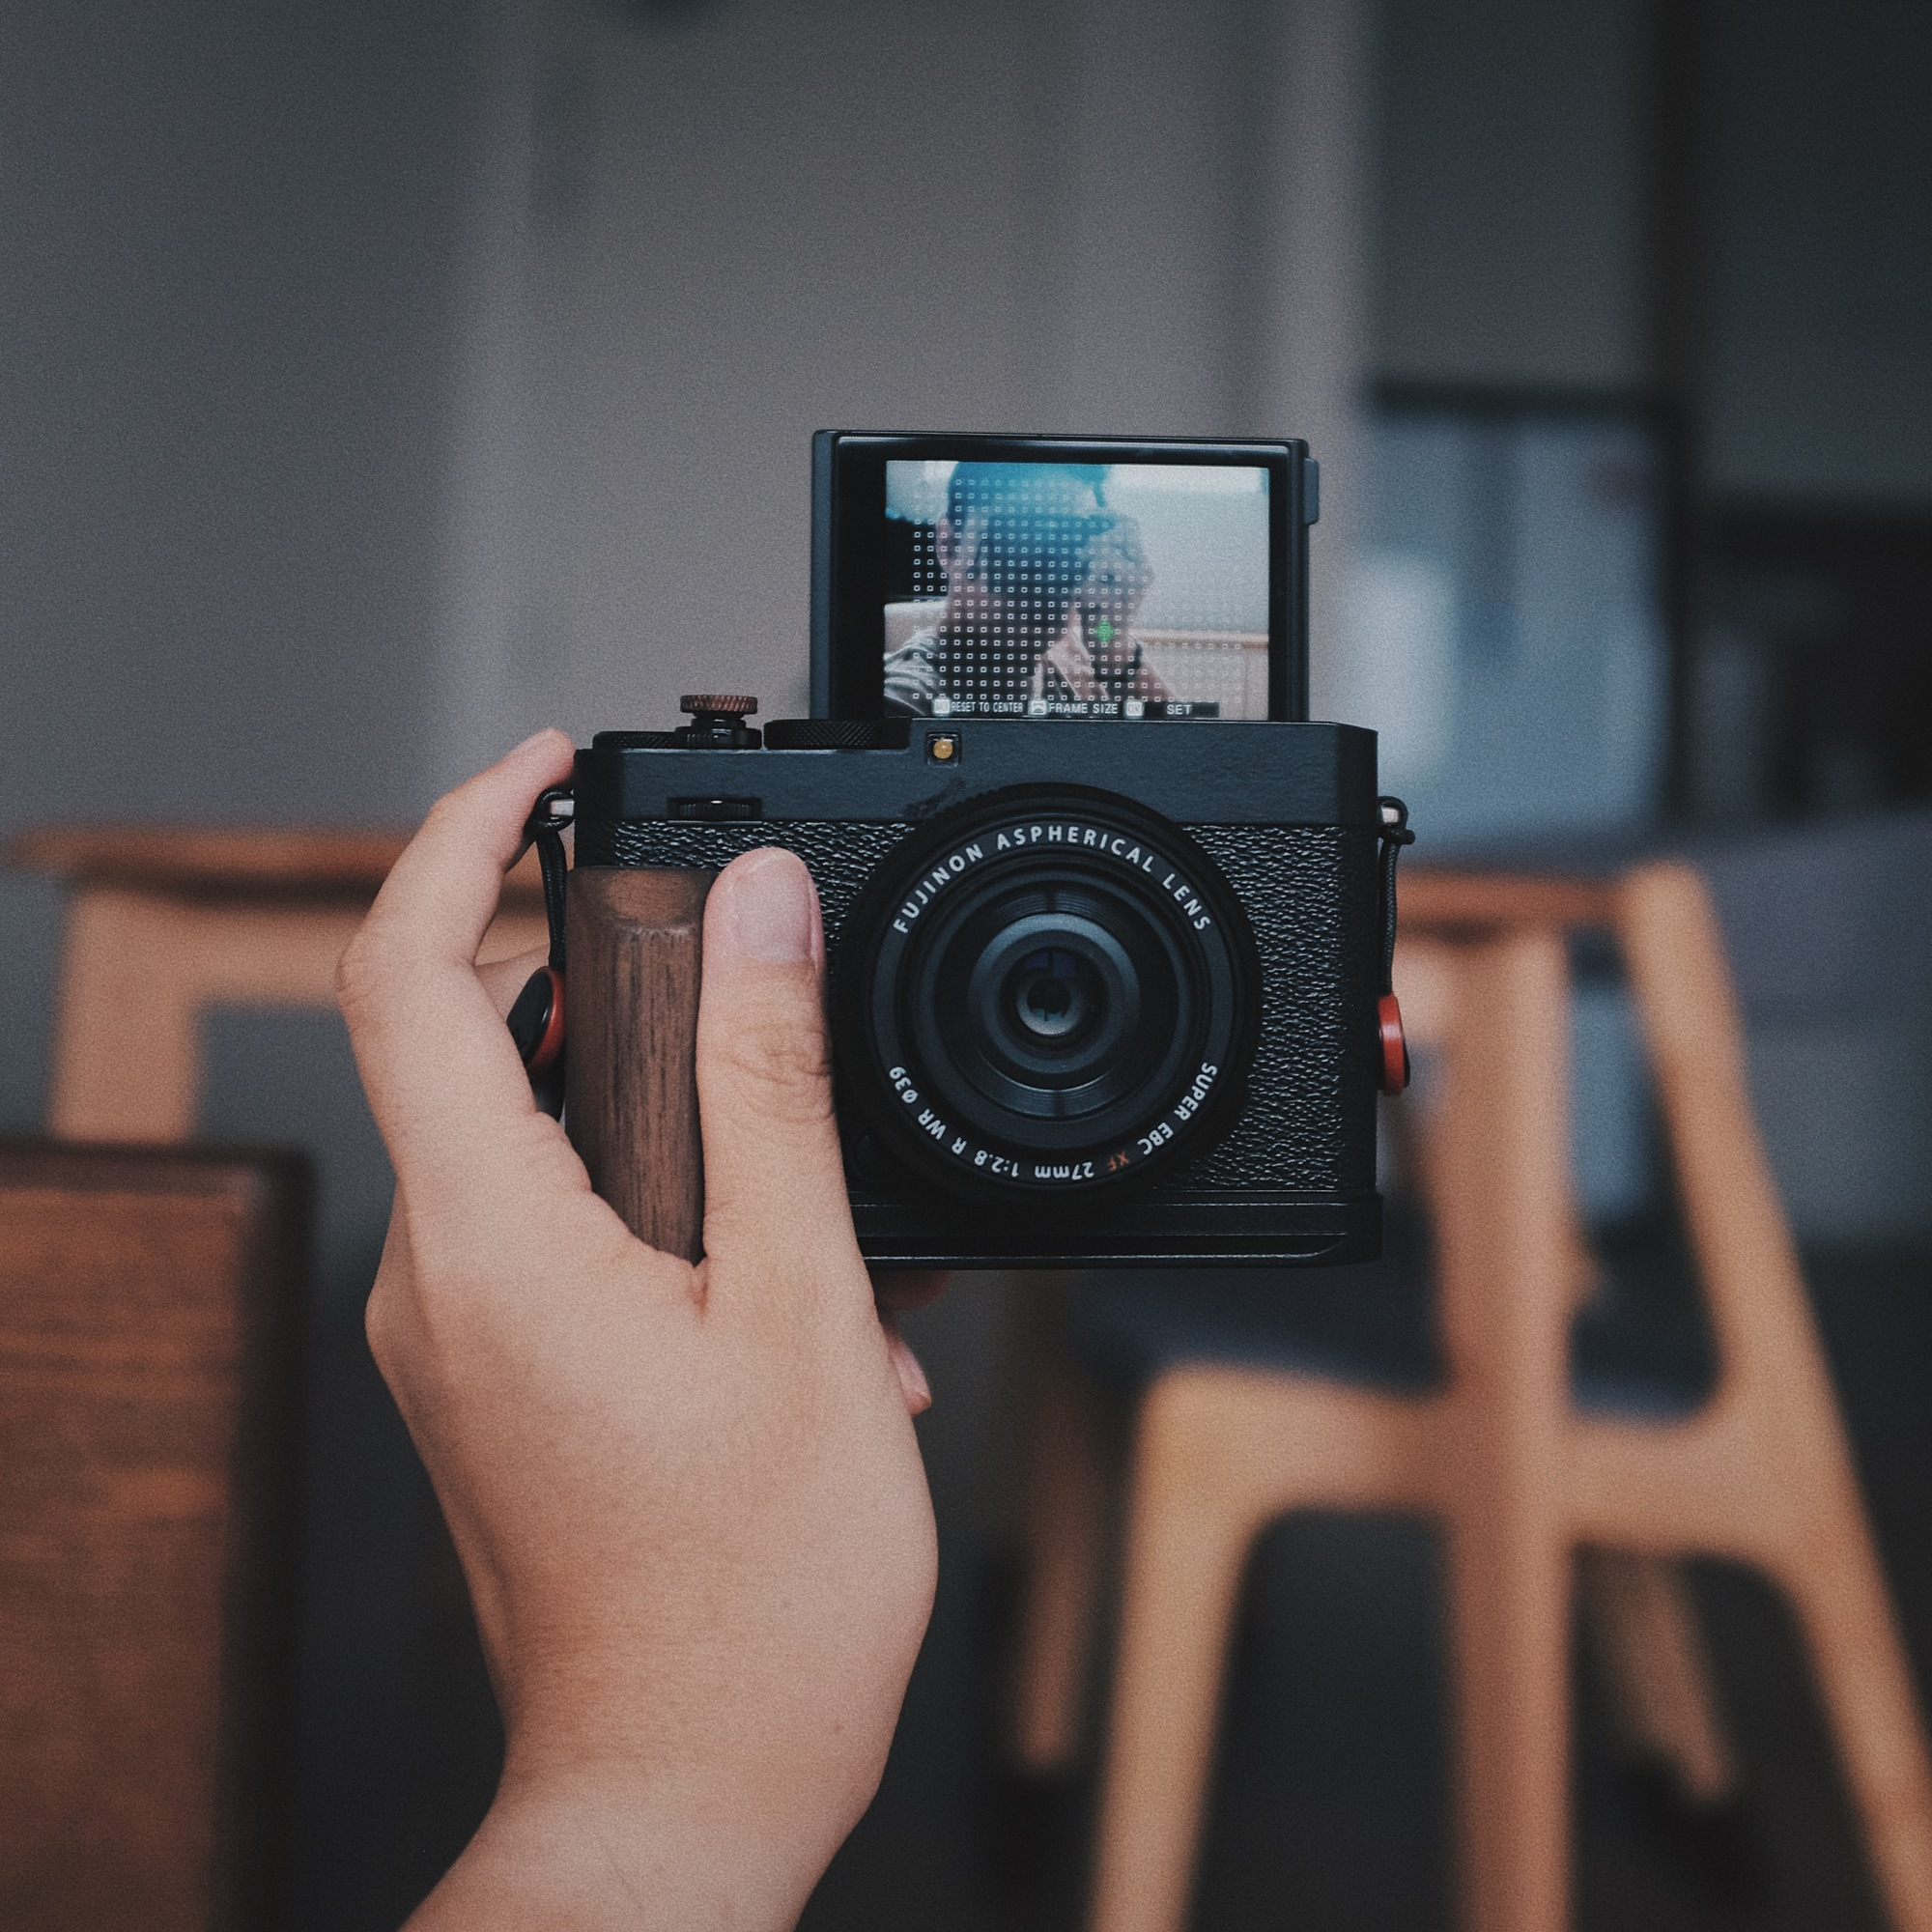
\includegraphics[width=\linewidth]{\envfinaldir/coverpic-prod.jpg}\par
            % \vskip 30pt
            \vfill

            \normalsize\rmfamily\scshape
            \copyright{} The Web Digest Project \hfill\large \envdatestr
        \end{center}
    \end{titlepage}
    % \restoregeometry
}
\newcommand{\simplehref}[1]{%
    \textcolor{blue!80!green}{\href{#1}{#1}}%
}
\renewcommand{\contentsname}{\center\Huge\sffamily\bfseries Contents\par\vskip 20pt}
\newcounter{ipartcounter}
\setcounter{ipartcounter}{0}
\newcommand{\ipart}[1]{
    % \vskip 20pt
    \clearpage
    \stepcounter{ipartcounter}
    \phantomsection
    \addcontentsline{toc}{chapter}{#1}
    % \begin{center}
    %     \Huge
    %     \sffamily\bfseries
    %     #1
    % \end{center}
    % \vskip 20pt plus 7pt
}
\newcounter{ichaptercounter}
\setcounter{ichaptercounter}{0}
\newcommand{\ichapter}[1]{
    % \vskip 20pt
    \clearpage
    \stepcounter{ichaptercounter}
    \phantomsection
    \addcontentsline{toc}{section}{\numberline{\arabic{ichaptercounter}}#1}
    \begin{center}
        \Huge
        \sffamily\bfseries
        #1
    \end{center}
    \vskip 20pt plus 7pt
}
\newcommand{\entrytitlefont}[1]{\subsection*{\raggedright\Large\sffamily\bfseries#1}}
\newcommand{\entryitemGeneric}[2]{
    % argv: title, url
    \parbox{\linewidth}{
        \entrytitlefont{#1}\par\vskip 5pt
        \footnotesize\ttfamily\mdseries
        \simplehref{#2}
    }\vskip 11pt plus 11pt minus 1pt
}
\newcommand{\entryitemGithub}[3]{
    % argv: title, url, desc
    \parbox{\linewidth}{
        \entrytitlefont{#1}\par\vskip 5pt
        \footnotesize\ttfamily\mdseries
        \simplehref{#2}\par\vskip 5pt
        \small\rmfamily\mdseries#3
    }\vskip 11pt plus 11pt minus 1pt
}
\newcommand{\entryitemAp}[3]{
    % argv: title, url, desc
    \parbox{\linewidth}{
        \entrytitlefont{#1}\par\vskip 5pt
        \footnotesize\ttfamily\mdseries
        \simplehref{#2}\par\vskip 5pt
        \small\rmfamily\mdseries#3
    }\vskip 11pt plus 11pt minus 1pt
}
\newcommand{\entryitemHackernews}[3]{
    % argv: title, hnurl, rawurl
    % \parbox{\linewidth}{
    %     \entrytitlefont{#1}\par\vskip 5pt
    %     \footnotesize\ttfamily\mdseries
    %     \simplehref{#3}\par
    %     \textcolor{black!50}{\href{#2}{#2}}
    % }\vskip 11pt plus 11pt minus 1pt
    \begin{minipage}{\linewidth}
            \entrytitlefont{#1}\par\vskip 5pt
            \footnotesize\ttfamily\mdseries
            \simplehref{#3}\par
            \textcolor{black!50}{\href{#2}{#2}}
    \end{minipage}\par\vskip 11pt plus 11pt minus 1pt
}







\begin{document}

\makeheader

\tableofcontents\clearpage




\ipart{Developers}
\ichapter{Hacker News}
\entryitemTwoLinks{Toronto man creates tiny mobile homes to help unhoused people escape the cold}{https://news.ycombinator.com/item?id=42541173}{https://www.cbc.ca/lite/story/1.7419805}

\entryitemTwoLinks{I was wrong about the ethics crisis}{https://news.ycombinator.com/item?id=42540862}{https://cacm.acm.org/opinion/i-was-wrong-about-the-ethics-crisis/}

\entryitemTwoLinks{How China turns members of its diaspora into spies}{https://news.ycombinator.com/item?id=42540427}{https://www.economist.com/china/2024/12/26/how-china-turns-members-of-its-diaspora-into-spies}

\entryitemTwoLinks{The Average American Spent 2.5 Months on Their Phone in 2024}{https://news.ycombinator.com/item?id=42539474}{https://www.pcmag.com/articles/yikes-the-average-american-spent-25-months-on-their-phone-in-2024}

\entryitemTwoLinks{We've not been trained for this: life after the Newag DRM disclosure [video]}{https://news.ycombinator.com/item?id=42538914}{https://media.ccc.de/v/38c3-we-ve-not-been-trained-for-this-life-after-the-newag-drm-disclosure}

\entryitemTwoLinks{38C3: Illegal Instructions}{https://news.ycombinator.com/item?id=42537631}{https://media.ccc.de/c/38c3}

\entryitemTwoLinks{WebGL Fluid Simulation}{https://news.ycombinator.com/item?id=42537567}{https://paveldogreat.github.io/WebGL-Fluid-Simulation/}

\entryitemTwoLinks{Personal Mail Server on OpenBSD (2019)}{https://news.ycombinator.com/item?id=42536750}{https://nicolascarpi.github.io/openbsd/2019/04/03/openbsd-mail-server.html}

\entryitemTwoLinks{Jeju Air Jet Crashes in South Korea With Over 170 Dead or Missing}{https://news.ycombinator.com/item?id=42536647}{https://www.bloomberg.com/news/articles/2024-12-29/plane-crashes-at-s-korea-airport-killing-at-least-23-yonhap}

\entryitemTwoLinks{38C3: Blinkencity, radio controlling street lamps and power plants [video]}{https://news.ycombinator.com/item?id=42535622}{https://media.ccc.de/v/38c3-blinkencity-radio-controlling-street-lamps-and-power-plants}

\entryitemTwoLinks{All You Need Is 4x 4090 GPUs to Train Your Own Model}{https://news.ycombinator.com/item?id=42535453}{https://sabareesh.com/posts/llm-rig/}

\entryitemTwoLinks{Finding and exploiting hidden features of Animal Crossing's NES emulator (2018)}{https://news.ycombinator.com/item?id=42535333}{https://jamchamb.net/2018/07/11/animal-crossing-nes-emulator-hacks.html}

\entryitemTwoLinks{Fish 4.0: The Fish of Theseus}{https://news.ycombinator.com/item?id=42535217}{https://fishshell.com/blog/rustport/}

\entryitemTwoLinks{Intel's \$475M error: the silicon behind the Pentium division bug}{https://news.ycombinator.com/item?id=42535071}{https://www.righto.com/2024/12/this-die-photo-of-pentium-shows.html}

\entryitemTwoLinks{Family of OpenAI whistleblower Suchir Balaji demand FBI investigate death}{https://news.ycombinator.com/item?id=42535057}{https://www.theguardian.com/us-news/2024/dec/28/openai-whistleblower-suchir-balaji}

\entryitemTwoLinks{Show HN: Anki AI Utils}{https://news.ycombinator.com/item?id=42534931}{https://github.com/thiswillbeyourgithub/AnkiAIUtils}

\entryitemTwoLinks{EU law mandating universal chargers for devices comes into force}{https://news.ycombinator.com/item?id=42534851}{https://www.france24.com/en/europe/20241228-eu-law-mandating-universal-chargers-for-devices-comes-into-force}

\entryitemTwoLinks{Apple Photos phones home on iOS 18 and macOS 15}{https://news.ycombinator.com/item?id=42533685}{https://lapcatsoftware.com/articles/2024/12/3.html}

\entryitemTwoLinks{Google's Results Are Infested, Open AI Is Using Their Playbook from the 2000s}{https://news.ycombinator.com/item?id=42532441}{https://chuckwnelson.com/blog/google-search-results-infested-open-ai-using-google-playbook}

\entryitemTwoLinks{U.S. homelessness jumps to record high amid affordable housing shortage}{https://news.ycombinator.com/item?id=42532311}{https://www.npr.org/2024/12/27/nx-s1-5241115/us-homeless-hud-housing-costs-migrants}\ichapter{Phoronix}
\entryitemGeneric{\hskip 0pt{}Benchmarking The AMD INVLPGB Linux Kernel Patches For Better Performance}{https://www.phoronix.com/review/amd-invlpgb-linux}

\entryitemGeneric{\hskip 0pt{}Kdenlive Preparing For An Exciting 2025 With Background Removal Tool \& More}{https://www.phoronix.com/news/Kdenlive-Background-Removal-25}

\entryitemGeneric{\hskip 0pt{}Faster USB Performance For xHCI DbC Coming With Linux 6.14 Plus A 10 Year Old Bug Fixed}{https://www.phoronix.com/news/Faster-USB-xHCI-DbC-Linux-6.14}

\entryitemGeneric{\hskip 0pt{}Ubuntu's Great Year From 24.04 LTS To Focusing More On Performance Optimizations}{https://www.phoronix.com/news/Ubuntu-2024-Great-Year}

\entryitemGeneric{\hskip 0pt{}Fish Shell Outlines Their Successes \& Challenges Going From C++ To Rust}{https://www.phoronix.com/news/Fish-Shell-Rust-Challenges}

\entryitemGeneric{\hskip 0pt{}Apple DWI Backlight Linux Driver Updated For Various iPhones, iPods \& iPads}{https://www.phoronix.com/news/Apple-DWI-Backlight-Linux-v4}

\entryitemGeneric{\hskip 0pt{}Linux 6.13-rc5 To See Fix For Intel TDX CoCo VMs Potentially Leaking Decrypted Memory}{https://www.phoronix.com/news/Linux-6.13-Fixing-TDX-CoCo-Leak}

\entryitemGeneric{\hskip 0pt{}NVIDIA Made Great Strides With Their Open-Source Kernel Code \& Wayland Support In 2024}{https://www.phoronix.com/news/NVIDIA-2024-Linux-Highlights}

\entryitemGeneric{\hskip 0pt{}A "Safe C++" Being Explored Using The New ClangIR}{https://www.phoronix.com/news/RFC-Safe-CXX-Using-ClangIR}


\ipart{Developers~~~~(zh-Hans)}
\ichapter{Solidot}
\entryitemGeneric{\hskip 0pt{}大众 80 万电动汽车车主的行踪短暂暴露在互联网上}{https://www.solidot.org/story?sid=80179}

\entryitemGeneric{\hskip 0pt{}Do Kwon 被批准引渡到美国受审}{https://www.solidot.org/story?sid=80178}

\entryitemGeneric{\hskip 0pt{}OpenAI 公布转变为营利性公司的计划}{https://www.solidot.org/story?sid=80177}

\entryitemGeneric{\hskip 0pt{}导弹是当今客机的最大杀手}{https://www.solidot.org/story?sid=80176}

\entryitemGeneric{\hskip 0pt{}科学家发现七个与短睡眠相关的突变基因}{https://www.solidot.org/story?sid=80175}

\entryitemGeneric{\hskip 0pt{}马斯克移除了 Laura Loomer 的蓝标}{https://www.solidot.org/story?sid=80174}

\entryitemGeneric{\hskip 0pt{}微软与 OpenAI 谈判将 AGI 定义为能产生千亿美元利润的系统}{https://www.solidot.org/story?sid=80173}

\entryitemGeneric{\hskip 0pt{}创业公司准备推出延长狗命的药物}{https://www.solidot.org/story?sid=80172}

\entryitemGeneric{\hskip 0pt{}研究显示东亚湖泊中的汞累积呈上升趋势}{https://www.solidot.org/story?sid=80171}

\entryitemGeneric{\hskip 0pt{}亚洲中产在变胖}{https://www.solidot.org/story?sid=80170}

\entryitemGeneric{\hskip 0pt{}天文学家发现至今最遥远的蝎虎BL型类星体}{https://www.solidot.org/story?sid=80169}

\entryitemGeneric{\hskip 0pt{}Windows 11 安装媒介 Bug 会导致安全更新失败}{https://www.solidot.org/story?sid=80168}

\entryitemGeneric{\hskip 0pt{}终端模拟器 Ghostty 释出 1.0 版本}{https://www.solidot.org/story?sid=80167}

\entryitemGeneric{\hskip 0pt{}微软在 Microsoft 365 中集成 AI 然后涨价}{https://www.solidot.org/story?sid=80166}\ichapter{V2EX}
\entryitemGeneric{\hskip 0pt{}[Apple] 大家说一些 mac 平台上非常想要的 win app 吧}{https://www.v2ex.com/t/1101126}

\entryitemGeneric{\hskip 0pt{}[阅读] 20241230.03:16《人类简史读书笔记》作者 S-Yilon}{https://www.v2ex.com/t/1101125}

\entryitemGeneric{\hskip 0pt{}[Surge] 打开 Surge 的增强模式之后导致内网的 VLAN 不通,求解决办法}{https://www.v2ex.com/t/1101124}

\entryitemGeneric{\hskip 0pt{}[天黑以后] 20241230 午夜俱乐部}{https://www.v2ex.com/t/1101122}

\entryitemGeneric{\hskip 0pt{}[问与答] 开启 cloudflare 小云朵后无法访问.}{https://www.v2ex.com/t/1101121}

\entryitemGeneric{\hskip 0pt{}[问与答] 冬天如何对抗静电}{https://www.v2ex.com/t/1101120}

\entryitemGeneric{\hskip 0pt{}[分享创造] 感谢 cursor,让我一个不懂前端的人也能设计出来像样的网站了}{https://www.v2ex.com/t/1101119}

\entryitemGeneric{\hskip 0pt{}[问与答] 求教,自己搭了个节点加中转用来给人做跨境电商的,有部分网页打不开}{https://www.v2ex.com/t/1101118}

\entryitemGeneric{\hskip 0pt{}[北京] 小道消息,1 月份开始五环外解除限购了}{https://www.v2ex.com/t/1101117}

\entryitemGeneric{\hskip 0pt{}[问与答] firefox 不能同步其他电脑端的书签?}{https://www.v2ex.com/t/1101116}

\entryitemGeneric{\hskip 0pt{}[互联网] iOS 和 iPadOS 在线观看高码率视频卡顿的原因究竟是什么?}{https://www.v2ex.com/t/1101115}

\entryitemGeneric{\hskip 0pt{}[问与答] 大家都是在哪里刷面试题的?}{https://www.v2ex.com/t/1101114}

\entryitemGeneric{\hskip 0pt{}[问与答] 为什么有些超市的无糖罐装可口可乐,单卖的价格比六连包的价格还便宜?}{https://www.v2ex.com/t/1101112}

\entryitemGeneric{\hskip 0pt{}[分享创造] Lokica :高效管理浏览器标签页、书签和历史记录必备神器}{https://www.v2ex.com/t/1101111}

\entryitemGeneric{\hskip 0pt{}[OpenWrt] openwrt 如何配置 IP 地址段分流,让中国 IP 走 WAN 1,而中国以外的 IP 地址段走 WAN 2?}{https://www.v2ex.com/t/1101110}

\entryitemGeneric{\hskip 0pt{}[macOS] [求助贴] MacBook 输入密码无法开机, 恢复模式无法进入}{https://www.v2ex.com/t/1101108}

\entryitemGeneric{\hskip 0pt{}[macOS] macOS Safari 非常不完善的下载功能}{https://www.v2ex.com/t/1101107}

\entryitemGeneric{\hskip 0pt{}[随想] 「公益」想要做一款「两岸寻亲」相关的 Wechat MINI App,希望能够找到小伙伴一起参与!}{https://www.v2ex.com/t/1101106}

\entryitemGeneric{\hskip 0pt{}[OpenAI] chatgpt 降智似乎不是我们能左右的}{https://www.v2ex.com/t/1101105}

\entryitemGeneric{\hskip 0pt{}[Swift] 分享个基于 UICollectionView 封装的数据驱动和声明式组件库 ListKit}{https://www.v2ex.com/t/1101104}

\entryitemGeneric{\hskip 0pt{}[问与答] 记账第一年,很有收获,分享一下账单,不知 v 友们花了多少}{https://www.v2ex.com/t/1101103}

\entryitemGeneric{\hskip 0pt{}[问与答] 有什么好用的电视源以及如何远程更新电视?}{https://www.v2ex.com/t/1101102}

\entryitemGeneric{\hskip 0pt{}[旅行] 去日本旅游十天,顺便买点啥可以回点血赚个机票钱呢?}{https://www.v2ex.com/t/1101101}

\entryitemGeneric{\hskip 0pt{}[Apple] Mac mini 到了,准备配个鼠标,推荐罗技 Master 3s 还是 Anywhere 3s 呢?}{https://www.v2ex.com/t/1101098}

\entryitemGeneric{\hskip 0pt{}[程序员] 国内找海外的远程工作靠谱吗?}{https://www.v2ex.com/t/1101097}

\entryitemGeneric{\hskip 0pt{}[程序员] 从 AI 辅助编程认识到了什么}{https://www.v2ex.com/t/1101096}

\entryitemGeneric{\hskip 0pt{}[分享发现] 天气 app-IOS 推荐 today weather}{https://www.v2ex.com/t/1101095}

\entryitemGeneric{\hskip 0pt{}[程序员] 安卓手机无法登录自建的 vaultwarden}{https://www.v2ex.com/t/1101094}

\entryitemGeneric{\hskip 0pt{}[问与答] 各位大佬,打算买空调,因为各种原因错过了国补,发现 pdd 上空调跟国补价格差不多,不过绝大部分都是那种黑标的 [品牌] ,进去了连店铺都看不到,不知道靠不靠谱啊,会不会卖了就跑路啊,有点心里没底。}{https://www.v2ex.com/t/1101093}

\entryitemGeneric{\hskip 0pt{}[问与答] 宽带没有 IPv6 应该怎么解决?}{https://www.v2ex.com/t/1101090}

\entryitemGeneric{\hskip 0pt{}[macOS] macOS Sequoia 15 怎么启用允许``任何来源''?  而且有时候从 github 下的软件必须用终端命令 xattr -cr 打开软件}{https://www.v2ex.com/t/1101088}

\entryitemGeneric{\hskip 0pt{}[生活] 婚姻问题想请教大佬们的看法}{https://www.v2ex.com/t/1101085}

\entryitemGeneric{\hskip 0pt{}[奇思妙想] 感觉以后是教培的天下}{https://www.v2ex.com/t/1101084}

\entryitemGeneric{\hskip 0pt{}[Android] 如何去学习和了解后端开发流程呢?}{https://www.v2ex.com/t/1101083}

\entryitemGeneric{\hskip 0pt{}[前端开发] 求助: 当使用 Angular 的 MatIcon 时,有概率不显示 icon 或者只显示部分的.}{https://www.v2ex.com/t/1101082}

\entryitemGeneric{\hskip 0pt{}[程序员] XXL-RPC v1.8.0 | 分布式服务框架}{https://www.v2ex.com/t/1101081}

\entryitemGeneric{\hskip 0pt{}[iPhone] ios 闹钟每日重置问题}{https://www.v2ex.com/t/1101079}

\entryitemGeneric{\hskip 0pt{}[问与答] 求推荐适合写代码用的小屏}{https://www.v2ex.com/t/1101078}

\entryitemGeneric{\hskip 0pt{}[程序员] 询问 windsurf 添加 rule 技巧}{https://www.v2ex.com/t/1101077}

\entryitemGeneric{\hskip 0pt{}[Windows] windows 如何防止浏览器弹窗或者中招?}{https://www.v2ex.com/t/1101076}

\entryitemGeneric{\hskip 0pt{}[问与答] [不懂就问] 山姆副卡换绑,换不了?}{https://www.v2ex.com/t/1101075}

\entryitemGeneric{\hskip 0pt{}[前端开发] 有趣的开源项目推荐}{https://www.v2ex.com/t/1101074}

\entryitemGeneric{\hskip 0pt{}[优惠信息] 邮储 app 搜秒杀, 6 大毛立减金}{https://www.v2ex.com/t/1101073}

\entryitemGeneric{\hskip 0pt{}[程序员] 为什么这么简单的一个问题,所有不联网的 AI 全部都答错了}{https://www.v2ex.com/t/1101072}

\entryitemGeneric{\hskip 0pt{}[分享发现] 从一件小事上窥见淘宝被 PDD 超过的原因之一。}{https://www.v2ex.com/t/1101071}

\entryitemGeneric{\hskip 0pt{}[信息安全] Nginx Proxy Manager 好像不太安全?几百个 CVE 漏洞...}{https://www.v2ex.com/t/1101070}

\entryitemGeneric{\hskip 0pt{}[问与答] (虚心请教)在会 Python 的情况下,是不是应该学习一下 RPA 互补好}{https://www.v2ex.com/t/1101069}

\entryitemGeneric{\hskip 0pt{}[程序员] 300 元价位无线路由器}{https://www.v2ex.com/t/1101068}

\entryitemGeneric{\hskip 0pt{}[程序员] 有没有开源的中转卖 API 的项目}{https://www.v2ex.com/t/1101067}

\entryitemGeneric{\hskip 0pt{}[程序员] 为什么几乎所有观察者模式的实现代码都是用副作用实现的?}{https://www.v2ex.com/t/1101064}


\ipart{Generic News}
\ichapter{AP News}
\entryitemWithDescription{\hskip 0pt{}Charles Dolan, HBO and Cablevision founder, dies at 98}{https://apnews.com/article/bc5b48318f336f633b7df006afcd60c4}{}

\entryitemWithDescription{\hskip 0pt{}Belgium will ban sales of disposable e-cigarettes in a first for the EU}{https://apnews.com/article/7726f7852994e9d4911ea9ce94b25e7a}{}

\entryitemWithDescription{\hskip 0pt{}Snoop's game: Snoop Dogg thrills the crowd in the bowl that bears his name}{https://apnews.com/article/8968731ee88f4ee79ce810b4bcbdb3fd}{}

\entryitemWithDescription{\hskip 0pt{}Mavs star Luka Doncic is latest pro athlete whose home was burglarized, business manager says}{https://apnews.com/article/ee7c7848c20deb9aa0b73b7a643ee4b9}{}

\entryitemWithDescription{\hskip 0pt{}Victor Wembanyama plays 1-on-1 chess with fans in New York}{https://apnews.com/article/a5d6ba5c1e1bfe9d44a853c5d156c389}{}

\entryitemWithDescription{\hskip 0pt{}Norwegian chess grandmaster Magnus Carlsen quits a tournament in a dispute over jeans}{https://apnews.com/article/7040b103edb8813a7d145319845fce0a}{}

\entryitemWithDescription{\hskip 0pt{}Trailblazing model Dayle Haddon dies from suspected carbon monoxide poisoning}{https://apnews.com/article/bedff81dcfd119cf2dd398518a771705}{}

\entryitemWithDescription{\hskip 0pt{}2 Oregon men die from exposure in a forest after they went out to look for Sasquatch}{https://apnews.com/article/3ab2a21c723e96f327b1f3fa53a1658e}{}

\entryitemWithDescription{\hskip 0pt{}Going out for New Year's? Most people say they've got better plans, according to an AP-NORC poll}{https://apnews.com/article/100dda9a1cd1c575e76696ad0f381c45}{}

\entryitemWithDescription{\hskip 0pt{}Olivia Hussey, star of the 1968 film `Romeo and Juliet,' dies at 73}{https://apnews.com/article/7f4510db63e17566491a03622a37fd40}{}

\entryitemWithDescription{\hskip 0pt{}Hundreds gathered in Hong Kong for the city's first pyrotechnics drone show}{https://apnews.com/article/8617cd6bdac0c611a23b2b5c701bb3d0}{}

\entryitemWithDescription{\hskip 0pt{}South African retrospective exhibition honors the colorful work of artist Esther Mahlangu}{https://apnews.com/article/be15dbfafa39ea6b58743845b436e0b2}{}

\entryitemWithDescription{\hskip 0pt{}Sportscaster Greg Gumbel dies from cancer at age 78}{https://apnews.com/article/ace2925dbb23282079fb2dba06efe9bb}{}\ichapter{联合早报}
\entryitemWithDescription{沈泽玮:台湾冲突阻遏法案只叫不咬?}{https://www.zaobao.com/news/china/story20240918-4758889}{美国众议院9月9日开启了长达一星期的``中国周'',共通过25项主要涉华法案。(法新社) 美国众议院在当地时间9月9日开启了长达一星期的``中国周'',在美国总统和国会选举举行之前,密集表决数十项与中国有关的法案,共通过25项主要涉华法案……}

\entryitemWithDescription{欧盟电动车关税投票倒计时 中国在分歧中寻支持}{https://www.zaobao.com/news/china/story20240917-4758953}{欧盟27个成员国将于9月25日就是否继续对进口自中国的电动汽车额外征税进行最后表决。图为上海港等待装运出口的电动汽车。(彭博社) 欧盟对中国电动汽车加征关税的投票进入倒计时,正在欧洲访问的中国商务部部长王文涛与欧盟多国政府高层就此进行协商,试图在立场分歧的成员国中争取到更多支持。 受访学者研判,欧盟对中国电动汽车加征关税不可避免,但具体的加税方式和幅度仍有一定弹性,这是王文涛此行与各国谈判的重点……}

\entryitemWithDescription{港府今年将举办逾400项国庆活动}{https://www.zaobao.com/news/china/story20240917-4759341}{再过十多天就是中国国庆75周年,香港天星小轮展示``国庆75周年''\,``三天免费搭小轮''等标语迎国庆。(中新社) 再过十多天就是中国国庆75周年,香港特区政府今年将举办逾400项庆祝活动,希望通过一连串活动庆祝国庆,并且弘扬爱国主义教育及刺激消费。 港府星期二(9月17日)召开记者会,介绍各项庆祝国庆活动和特别优惠,涉及出行及吃喝玩乐等领域……}

\entryitemWithDescription{美空军部长:中国大陆军演精密化 为入侵封锁台湾做准备}{https://www.zaobao.com/news/china/story20240917-4759407}{美国空军部长肯德尔星期一(9月16日)在空军暨太空军协会的一场大会上致辞,提到中国对印太地区日益增长的威胁。(取自美国国防部网站) (华盛顿综合讯)美国空军部长肯德尔指,中国大陆军演的规模越来越大,也更加精密化,这是在专门为入侵、封锁台湾做准备。他也称,中国对印太地区的威胁现在已存在……}

\entryitemWithDescription{批准潜在对台备件军售案后 美派巡逻机过航台海}{https://www.zaobao.com/news/china/story20240917-4758770}{台军士兵8月26日在屏东县枋山训练场进行实弹演习时,从M1167 TOW运载车上发射一枚美制TOW-2A线导反坦克导弹。(路透社) (华盛顿/台北/北京综合讯)在批准潜在对台备件军售案之后,美国派遣反潜巡逻机过航台湾海峡,中国人民解放军东部战区则组织战机跟监美机,并誓言``坚决捍卫国家主权''……}

\entryitemWithDescription{李家超:若香港驻美经贸办被关 受害的是美企}{https://www.zaobao.com/news/china/story20240917-4758797}{香港特首李家超星期一(9月17日)警告,如果美国通过法案,导致香港驻美经贸办关闭,受害的是美国企业。图为李家超9月11日在``一带一路''高峰论坛上致辞。(彭博社) (香港综合讯)香港特首李家超警告,如果美国通过法案,导致香港驻美经贸办关闭,受害的是美国企业。 美国众议院上周通过《香港经济贸易办事处认证法案》,如果参议院也表决通过并交由总统签署成法,香港三个驻美国的经贸办可能将被强制关闭……}

\entryitemWithDescription{美国指中国航空工业集团员工企图实施黑客攻击}{https://www.zaobao.com/news/china/story20240917-4757988}{(华盛顿综合讯)中国航空航天巨头中国航空工业集团一名员工被指试图对美国宇航局、美国军方和其他目标展开黑客攻击。 据彭博社报道,美国检察官布坎南星期一(9月16日)在起诉书中,指控中国航空工业集团39岁的工程师吴宋(音译,Song Wu)企图从美国宇航局、空军、陆军和海军,以及联邦航空管理局取得电脑软件和源代码……}

\entryitemWithDescription{【东谈西论】恒大账务造假 普华永道是共犯还是被拖累?}{https://www.zaobao.com/news/china/story20240917-4756452}{因涉及恒大地产审计项目的违法行为,普华永道中国9月13日被中国财政部和证监会处以4.41亿人民币罚款并被令停业六个月, 广州分所被撤销……}

\entryitemWithDescription{戴庆成:香港输入人才计划大检阅}{https://www.zaobao.com/news/china/story20240917-4744978}{香港于2022年底推出高端人才通行证计划。(法新社) 2019年香港反修例风波过后,数以十万计港人移居海外,令香港出现人才荒。港府为了解决这个问题,在过去几年积极引入``新血'',当中以高才通计划最受瞩目,社会上也不时热议其成效。 高才通全称为高端人才通行证计划,于2022年底推出,申请人年收入须达到250万港元(约42万新元)以上,或本科毕业于全球百强大学并满足一定工作年限等……}

\entryitemWithDescription{中美希望稳定双边关系 中小国家可​​​搭建桥梁}{https://www.zaobao.com/news/china/story20240917-4745091}{中美元首去年11月在旧金山会晤后,双方都希望稳定两国关系,我国巡回大使陈庆珠认为,如果中美两国都认为走向战争不符合它们的利益,那么中小国家就可以做点什么,为双方搭建桥梁。 陈庆珠星期一(9月16日)在李光耀公共政策学院的一场研讨会上说,中国与西方的关系面对诸多困难,有中国智库表示,希望新加坡能协助在中美之间建立更多对话,``因为新加坡受美国信任,也在中国有渠道''……}

\entryitemWithDescription{陈庆珠:世界经历了三次``中国冲击'' 中美的主导力之争将继续}{https://www.zaobao.com/news/china/story20240917-4744996}{李光耀公共政策学院``思想之节庆''的一场研讨会,讨论``历史终结时的中国冲击''。左起是我国巡回大使陈庆珠、通商中国主席李奕贤、李光耀公共政策学院国际关系助理教授何莉菁、李光耀公共政策学院院长柯成兴……}

\entryitemWithDescription{上海遭遇75年来最强台风 扰乱民众中秋假期出行}{https://www.zaobao.com/news/china/story20240916-4745224}{台风贝碧嘉星期一(9月16日)登陆上海,维护人员星期一下午在衡山路上处理倒伏的树木。 (新华社) 台风造成上海上万株数目倒伏或折断。图为一棵倒下的大树砸坏一旁的建筑。(法新社) 台风贝碧嘉登陆上海后,黄浦江苏州河口潮位上涨,乌云密布。(中新社) 中国上海市星期一(9月16日)遭遇75年来最强台风``贝碧嘉''登陆,也是上海有记录以来首次有强台风侵袭……}

\entryitemWithDescription{陆男频长驱偷渡台湾在测试边防实力?}{https://www.zaobao.com/news/china/story20240916-4745161}{中国大陆一名王姓男子在中秋节前夕,乘橡皮艇从浙江宁波抵达台湾新北市林口,主动打电话投案,海巡署人员前去接他上岸。(自由時報) 中国大陆一名王姓男子划橡皮艇于上星期六清晨偷渡到台湾,隔天被新北市地方法院裁定羁押禁见。这是6月以来第二起大陆人士偷渡至台湾,此间专家质疑是否为海防破口,并怀疑对岸是否在测试台湾的边防实力……}

\entryitemWithDescription{中美时隔八月举行国防部工作会晤}{https://www.zaobao.com/news/china/story20240916-4745025}{(北京/华盛顿综合讯)中美双方上周末举行国防部工作会晤;美国官员称,美国积极进行美中两军外交活动,不代表美国对有关中国议题的处理方式发生任何改变。 据中国国防部星期天(15日)晚上通报,北京香山论坛结束后,第18次中美国防部工作会晤上星期六至星期天(9月14日至15日)在北京举行……}

\entryitemWithDescription{中国高校今年拟增足球运动本科专业}{https://www.zaobao.com/news/china/story20240916-4744925}{(北京综合讯)为了培养足球专业人才,中国大专学府今年度拟新增足球运动本科专业,以具体落实中国足球改革。 综合人民网和《南方都市报》报道,中国教育部上星期五(9月13日)发布《2024年度普通高等学校本科专业申报材料公示》。根据公示统计,今年度拟新增专业535个,涉及353所高校,其中39所高校新增足球运动专业……}

\entryitemWithDescription{香港23条首案 港男因穿``光时''上衣被定罪}{https://www.zaobao.com/news/china/story20240916-4743439}{(香港综合讯)香港一名无业男子,今年6月因穿印有2019年反修例抗争口号的上衣而被捕。他星期一承认违反煽动意图罪,成为在《维护国家安全条例》(即《香港基本法》第23条)下被定罪的第一人。 综合港媒《星岛日报》和路透社报道,27岁无业男子诸启邦今年6月12日在石门港铁站附近,未能出示身份证供查阅被警方拘捕……}

\entryitemWithDescription{美国务院:中国释放被关押近20年美籍牧师}{https://www.zaobao.com/news/china/story20240916-4744614}{(华盛顿综合电)中国释放被关押近20年的美国籍牧师,显示北京在中美关系的关键时刻展现善意。 综合彭博社、法新社和路透社报道,美国国务院发言人星期天(9月15日)说:``我们欢迎林大卫(音译,David Lin)从中华人民共和国的监狱获释。他已回返美国,这是他近20年来首次与家人见面。'' 林大卫的女儿艾丽斯告诉美国政治新闻网Politico,她的父亲将抵达得克萨斯州的圣安东尼奥……}

\entryitemWithDescription{中国驻泰使馆:近期并未向湄公河下游泄洪}{https://www.zaobao.com/news/china/story20240916-4743917}{(北京讯)泰国西北部的湄公河因洪水泛滥而决堤,中国否认这是中方泄洪所致,并称近来已持续减少云南景洪水电站的出库流量,以助下游地区抗洪。 中国驻泰国大使馆星期日(9月15日)深夜在官方微信公众号发文说,当天又有媒体报道称中国正在向湄公河泄洪,经向中国主管部门核实,使馆再次澄清,为帮助下游地区应对洪灾,中方近来持续稳定和减少景洪水电站出库流量,不可能对下游地区抗洪救灾形成压力……}

\entryitemWithDescription{加入美国储存可靠度评估计划 台湾军方编列预算采购三类型导弹}{https://www.zaobao.com/news/china/story20240916-4743826}{(台北讯)据台媒报道,台湾军方持续向美国采购可简易操作的导弹,预计在2024年、2031年以前获得400枚``标枪''反装甲导弹、2485枚``刺针''人携式防空导弹……}

\entryitemWithDescription{韩咏红:中美分头追逐全球南方}{https://www.zaobao.com/news/china/story20240916-4730719}{9月5日,中国外长王毅(中)同中非合作论坛非方现任共同主席国塞内加尔外长法勒(左)、下任共同主席国刚果外长加科索(右),在北京共同会见中外记者并答问。(路透社) 进入气候宜人的9月,中国接连举行了两场受瞩目的国际会议,一是聚集非洲53国国家元首与政要的中非合作论坛,接着是周末刚闭幕的北京香山论坛。 两场活动的参与者不同,规模也有很大差距……}

\entryitemWithDescription{菲律宾船只撤离中菲争议海域后 将再派船接替}{https://www.zaobao.com/news/china/story20240915-4730494}{这张在9月15日拍摄,并由菲律宾海岸警卫队提供的照片显示,菲律宾海岸警卫队船马格巴努亚号抵达了菲国巴拉望岛的一个港口。菲律宾早前以发现填海活动为由,今年4月派出马格巴努亚号前往萨比纳礁。(法新社/菲律宾海岸警卫队) 菲律宾国家海事委员会星期天(9月15日)发声明称,该国海岸警卫队一艘巡逻舰已离开萨比纳礁争议海域……}

\entryitemWithDescription{台风贝碧嘉直击中国华东 多趟本地与沪杭间航班取消}{https://www.zaobao.com/news/china/story20240915-4730611}{9月15日在上海外滩滨江步道上,一名外籍游客的雨伞被大风吹起。台风贝碧嘉的中心当天下午5时位于上海市东偏南方大约435公里的东海海面上,中心附近最大风力有13级。(中新社) (上海/新加坡综合讯)台风贝碧嘉预计将为中国华东沿海地区带来狂风暴雨,多趟往返新加坡与上海和杭州的航班取消……}






\clearpage
\leavevmode\vfill
\footnotesize

Copyright \copyright{} 2023-2024 Neruthes and other contributors.

This document is published with CC BY-NC-ND 4.0 license.

The entries listed in this newsletter may be copyrighted by their respective creators.

This newsletter is generated by the Web Digest project.

The newsletters are also delivered via Telegram channel \CJKunderline{\href{https://t.me/webdigestchannel}{https://t.me/webdigestchannel}}.\\
RSS feed is available at \CJKunderline{\href{https://webdigest.pages.dev/rss.xml}{https://webdigest.pages.dev/rss.xml}}.

This newsletter is available in PDF at
\CJKunderline{\href{https://webdigest.pages.dev/}{https://webdigest.pages.dev/}}.

The source code being used to generate this newsletter is available at\\
\CJKunderline{\href{https://github.com/neruthes/webdigest}{https://github.com/neruthes/webdigest}}.

This newsletter is also available in
\CJKunderline{\href{http://webdigest.pages.dev/readhtml/\envyear/WebDigest-20241229.html}{HTML}} and
\CJKunderline{\href{https://github.com/neruthes/webdigest/blob/master/markdown/\envyear/WebDigest-20241229.md}{Markdown}}.


\coverpic{https://unsplash.com/photos/unknown-person-stepping-on-brown-sand-agRHZWN95Ps}{Mollie Defibaugh}


\end{document}
